\subsection{INTEGRAL OF A LIMIT OF FUNCTIONS ON A NON-COMPACT INTERVAL}

Th. 1 of II, p.~52 applies to functions more general than regulated functions, since there one merely assumes that the functions admit primitives. In particular one sees that prop. 1 of II, p.~68 still applies when, on an interval I ⊂ R, the functions \(f_{\alpha}\) are only assumed to be piecewise regulated and to admit an integral over I; however this result presupposes that the other two hypotheses of prop. 1 are satisfied, namely: 1° I is a bounded interval; 2° the \(f_{\alpha}\) converge uniformly on I to f.~Formula (1) of II, p.~68 may fail when one of these conditions is no longer satisfied: it can happen that one or the other of these two terms does not exist, or that both exist but have different values.

For example, if \(f_{n}\) is the regulated function on {]}0, 1{]}, defined by \(f_{n}(x) = n\) for \(0 < x < 1 / n\) and \(f_{n}(x) = 0\) for \(1 / n \leqslant x \leqslant 1\) , then the sequence \((f_{n})\) converges to 0 uniformly on every compact interval contained in \([0, 1]\) , but not uniformly on \([0, 1]\) , and one has \(\int_{0}^{1} f_{n}(t) dt = 1\) for each n.~One has an example where \(\int_{0}^{1} f_{n}(t) dt\) does not tend to any limit on replacing the preceding sequence \((f_{n})\) by the sequence \(((-1)^{n} f_{n})\) which again converges uniformly to 0 on every compact interval contained in \([0, 1]\) .

On the other hand, on the unbounded interval I = {[}0, +∞{[}, let \(f_{n}\) be the regulated function such that \(f_{n}(x) = 1/n\) for \(n^{2} \leqslant x \leqslant (n+1)^{2}\) and \(f_{n}(x) = 0\) for every other value of x in I ( \(n \geqslant 1\) ); the sequence \((f_{n})\) converges uniformly to 0 on I, but the integral \(\int_{0}^{+\infty} f_{n}(t) dt = (2n+1)/n\) tends to 2 as n increases indefinitely.

\pandocbounded{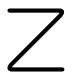
\includegraphics[keepaspectratio]{images/part001_bd86b8f3.jpg}}

In other words, when I is not bounded, if one denotes by \(\mathcal{I}\) the vector space formed by the regulated functions \(\mathbf{f}\) on I, with values in E, and admitting an integral over I, then the map \(\mathbf{f} \mapsto \int_{\mathrm{I}} \mathbf{f}(t) dt\) is not continuous when one endows \(\mathcal{I}\) with the topology of uniform convergence on I (cf.~II, p.~53, cor. 2).

We shall seek sufficient conditions to assure the validity of prop. 1, under the following hypotheses:

\(1^{\circ}\) I is an arbitrary interval in \(\mathbf{R}\) , the function \(\mathbf{f}_{\alpha}\) is regulated on I, and admits an integral over I;

\(2^{\circ}\) the family \((\mathbf{f}_{\alpha})\) converges uniformly to \(\mathbf{f}\) with respect to the filter \(\mathfrak{F}\) on every compact interval contained in I.

Writing \(\mathfrak{K}(\mathrm{I})\) for the directed set of compact intervals contained in I (II, p.~64), the left-hand side of formula (1) of II, p.~68 can be written as \(\lim_{\mathfrak{F}}\left(\lim_{\mathrm{J}\in \mathfrak{K}(\mathrm{I})}\int_{\mathrm{J}}\mathbf{f}_{\alpha}(t)dt\right)\) ; on
the other hand, taking account of prop. 1 (II, p.~68), and also the fact that the family \((\mathbf{f}_{\alpha})\) is uniformly convergent on every compact interval \(J \subset I\) , the right-hand side of (1) (II, p.~68) can be written as \(\lim_{\mathrm{J} \in \mathfrak{K}(\mathrm{I})} \left( \lim_{\mathfrak{F}} \int_{\mathrm{J}} \mathbf{f}_{\alpha}(t) dt \right)\) . One thus sees that prop. 1 of
II, p.~19 extends when one can interchange the limits of the map(J, \(\alpha\) ) \(\mapsto \int_{J} f_{\alpha}(t) dt\) with respect to the filter F and with respect to the filter \(\Phi\) of sections of the directed set K(I). Now, we know a sufficient condition for this interchange to be justified, namely the existence of the limit of the map (J, \(\alpha\) ) \(\mapsto \int_{J} f_{\alpha}(t) dt\) with respect to the product filter \(\Phi \times F\) (Gen.~Top., I, p.~81, cor. to th. 1). We shall transform this condition into an equivalent, more manageable, condition.

In the first place, since E is complete, in order that \((\mathbf{J}, \alpha) \mapsto \int_{\mathbf{J}} \mathbf{f}_{\alpha}(t) dt\) should have a limit with respect to \(\Phi \times F\) it is necessary and sufficient that, for every \(\varepsilon > 0\) , there should exist a compact interval \(J_{0} \subset I\) and a set \(M \in F\) such that, for any elements \(\alpha\) , \(\beta\) of M and compact interval \(J \supset J_{0}\) contained in I, one has

\[
\left\| \int_ {J _ {0}} \mathbf {f} _ {\alpha} (t) d t - \int_ {J} \mathbf {f} _ {\beta} (t) d t \right\| \leqslant \varepsilon .\tag{4}
\]

We shall show on the other hand that this condition is itself equivalent to the following condition: for every \(\varepsilon > 0\) there exists a compact interval \(J_0 \subset I\) and a set \(M \in \mathfrak{F}\) such that, for any \(\alpha\) of \(M\) and any compact interval \(J \supset J_0\) contained in \(I\) , one has

\[
\left\| \int_ {J _ {0}} \mathbf {f} _ {\alpha} (t) d t - \int_ {J} \mathbf {f} _ {\alpha} (t) d t \right\| \leqslant \varepsilon .\tag{5}
\]

It is indeed clear that this last condition is necessary; conversely, if it is satisfied, there exists (by the uniform convergence of \((\mathbf{f}_{\alpha})\) on every compact interval) a set \(N \in F\) such that, for any \(\alpha\) , \(\beta\) in N one has

\[
\left\| \int_ {\mathrm{J} _ {0}} \mathbf {f} _ {\alpha} (t) d t - \int_ {\mathrm{J} _ {0}} \mathbf {f} _ {\beta} (t) d t \right\| \leqslant \varepsilon ;\tag{6}
\]

and therefore \(\left\|\int_{J_{0}}\mathbf{f}_{\alpha}(t)dt-\int_{J}\mathbf{f}_{\beta}(t)dt\right\|\leqslant2\varepsilon\) for any \(\alpha\) and \(\beta\) in \(M\cap N\in\mathfrak{F}\) and for any compact interval \(J\supset J_{0}\) .

Finally, the lemma of II, p.~65 allows us to put this last condition in the following equivalent form: for every \(\varepsilon > 0\) there exist a compact interval \(\mathbf{J}_0 \subset \mathbf{I}\) and a set \(\mathbf{M} \in \mathfrak{F}\) (depending on \(\varepsilon\) ) such that, for every compact interval \(\mathbf{K} \subset \mathbf{I}\) having no interior point in common with \(\mathbf{J}_0\) , and every \(\alpha \in \mathbf{M}\) , one has \(\left\| \int_{\mathbf{K}} \mathbf{f}_{\alpha}(t) dt \right\| \leqslant \varepsilon\) .

Most often, one uses a more restrictive condition obtained by supposing that, in the last statement, the set M does not depend on \(\varepsilon\) :

DEFINITION 1. One says that the integral \(\int_{\mathrm{I}} \mathbf{f}_{\alpha}(t) dt\) is uniformly convergent for \(\alpha \in \mathrm{A}\) (or uniformly convergent over \(\mathrm{A}\) ) if, for every \(\varepsilon > 0\) there exists a compact interval \(\mathrm{J}_0 \subset J\) such that, for every compact interval \(\mathrm{K} \subset \mathrm{I}\) with no interior point in common with \(\mathrm{J}_0\) , and every \(\alpha \in \mathrm{A}\) , one has

\[
\left\| \int_ {K} \mathbf {f} _ {\alpha} (t) d t \right\| \leqslant \varepsilon .\tag{7}
\]

This definition is equivalent to saying that the family of maps \(\alpha\mapsto\int_{J}\mathbf{f}_{\alpha}(t)dt\) is uniformly convergent on A (towards the map \(\alpha\mapsto\int_{I}\mathbf{f}_{\alpha}(t)dt\) ) with respect to the filter of sections \(\Phi\) of \(\Re(I)\) ; each of the integrals \(\int_{I}\mathbf{f}_{\alpha}(t)dt\) is a fortiori convergent (the converse being false); Further, from what we have just seen (or from Gen.~Top., X, p.~281, cor. 2):

PROPOSITION 3. Let \((\mathbf{f}_{\alpha})\) be a family of regulated functions on an interval I such that: \(1^{\circ}\) with respect to the filter \(\mathfrak{F}\) the family \((\mathbf{f}_{\alpha})\) converges uniformly to a function \(\mathbf{f}\) (regulated on I) on every compact interval contained in I; \(2^{\circ}\) the integral \(\int_{I} \mathbf{f}_{\alpha}(t) dt\) is uniformly convergent for every \(\alpha \in A\) . Under these hypotheses the integral \(\int_{I} \mathbf{f}(t) dt\) is convergent, and one has

\[
\lim _ {\mathfrak {F}} \int_ {\mathrm{I}} \mathbf {f} _ {\alpha} (t) d t = \int_ {\mathrm{I}} \mathbf {f} (t) d t.\tag{8}
\]

The hypotheses of prop. 3 are fulfilled when for example I is a bounded interval, the \(\mathbf{f}_{\alpha}\) are uniformly bounded on I, and converge uniformly to \(\mathbf{f}\) on every compact interval contained in I; indeed, if \(\| \mathbf{f}_{\alpha}(x)\| \leqslant h\) for all \(x\in \mathrm{I}\) and all \(\alpha\) , and if \(\mathrm{J}_0\) is such that the difference between the lengths of I and \(\mathrm{J}_0\) is \(\leqslant \varepsilon /h\) , then condition (7) is satisfied for every interval \(\mathrm{K}\subset \mathrm{I}\) with no interior point in common with \(\mathrm{J}_0\) .

As with prop. 1 of II, p.~68, two corollaries to prop. 3 are important in applications:

COROLLARY 1. Let \((\mathbf{f}_{n})\) be a sequence of regulated functions on an arbitrary interval I, converging uniformly to a function f on each compact interval contained in I; if the integral \(\int_{I} \mathbf{f}_{n}(t) dt\) is uniformly convergent, then the integral \(\int_{I} \mathbf{f}(t) dt\) is convergent, and

\[
\lim _ {n \to \infty} \int_ {\mathrm{I}} \mathbf {f} _ {n} (t) d t = \int_ {\mathrm{I}} \mathbf {f} (t) d t.\tag{9}
\]

Remark. The hypotheses imposed in this corollary are sufficient, but not necessary, for the validity of formula (9); we shall generalize this formula later, at the same time as the concept of integral (see INT, IV), and obtain much less restrictive conditions.

COROLLARY 2. Let A be a subset of a topological space F, and f a map of I × A into a complete normed space E over R, such that, for every \(\alpha \in A\) , the function \(x \mapsto \mathbf{f}(x, \alpha)\) is regulated on I. If, on the one hand, the functions \(x \mapsto \mathbf{f}(x, \alpha)\) converge uniformly on every compact interval contained in I to a function \(x \mapsto \mathbf{f}(x)\) as \(\alpha\) tends to \(\alpha_{0} \in \overline{A}\) while remaining in A; if, on the other hand, the integral \(\int_{I} \mathbf{f}(x, \alpha) dx\) is uniformly convergent on A, then the integral \(\int_{I} \mathbf{f}(x) dx\) is convergent, and one has

\[
\lim _ {\alpha \rightarrow \alpha_ {0}, \alpha \in A} \int_ {I} \mathbf {f} (x, \alpha) d x = \int_ {I} \mathbf {f} (x) d x.\tag{10}
\]

In particular:

PROPOSITION 4 (``continuity of an improper integral with respect to a parameter''). Let F be a compact space, let I be any interval in R, and f a continuous map from I × F into a complete normed space E over R; if the integral \(\mathbf{h}(\alpha) = \int_{\mathrm{I}} \mathbf{f}(x, \alpha) dx\) is uniformly convergent on F, it is a continuous function of \(\alpha\) on F.

In view of prop. 2 of II, p.~69, this proposition also follows from the continuity of a uniform limit of continuous functions (Gen.~Top., X, p.~282, th. 2).

